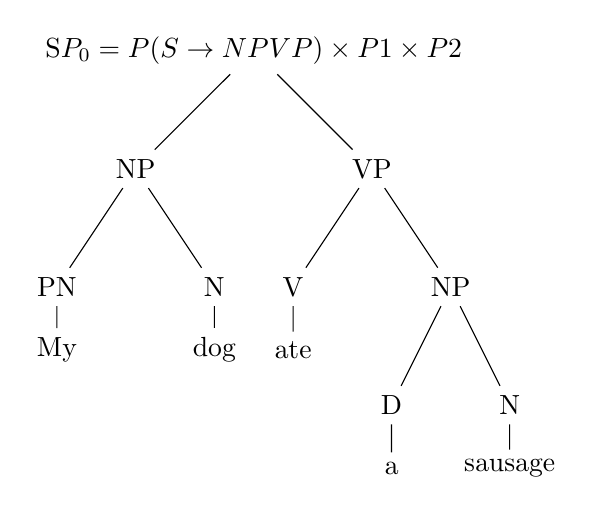
\begin{tikzpicture}
\tikzstyle{level 1}=[sibling distance=30mm]
\tikzstyle{level 2}=[sibling distance=20mm]
\tikzstyle{level 3}=[sibling distance=15mm]
\node {S\\$P_0 = P(S\rightarrow NP VP)\times P1\times P2$} 
	child {node (leftnode) {NP}
		child {node {PN}
			child  [level distance = 8mm] {node {My}}
			}
		child {node {N}
			child[level distance = 8mm] {node {dog}}
			}
		}
	child {node (rightnode) {VP}
		child {node {V}
			child[level distance = 8mm]{node {ate}}
			}
		child {node {NP}
			child {node {D}
				child[level distance = 8mm]{node {a}}
				}
			child { node {N}
				child[level distance = 8mm]{node {sausage}}
				}
			}
		} ;


\end{tikzpicture}
\caption{The probability of a tree is a multiplication of the probability of the production with the probability of its children}